\documentclass{article}
\usepackage[margin=1in]{geometry}
\usepackage{microtype}
\usepackage{setspace}
\usepackage{amsmath}
\usepackage{parskip}
\usepackage{amssymb}
\usepackage{graphicx}

\graphicspath{{../public/}}

\parskip=4ex
\date{}
\author{}

\title{12.5 Triple Integrals}

\begin{document}
  \maketitle
  Triple integrals are functions of three variables. The simplest case is where $ f $   is defined on a rectangular box
  \[
    B= \{ (x,yz) | a\le x \le b, c \le y \le d, r \le z \le s \}
  \]
  
  As always the region, in this case, $ B $ is divided into sub-boxes. Done by dividing the interval $ [a,b] $ into $ l $ subintervals $ [x_{i-1},x_i] $ with lengths $ \Delta x_i=x_i - x_{i-1} $, dividng $ [c,d] $ into $ m $ subintervals with lengths $ \Delta y_j=y_j-y_{j-1} $, and dividing $ [r,s] $ into $ n $ subintervals with lengths $ \Delta z_k=z_k-z_{k-1} $. The planes through the endpoints of these subintervals parallel to the coordinate planes divide the box $ B $ into $ lmn $ sub-boxes
  \[
    B_{ijk}=[x_{i-1},x_i] \times [y_{j-1},y_j] \times [z_{k-1},z_k]
  \]

  As shown below. The sub-box $ B_{ijk} $ has volume $ \Delta V_{ijk}=\Delta x_i \Delta y_j \Delta z_k $ 

  Which can be used to form the triple Riemann sum
  \[
    \sum^{l}_{i=1} \sum^{m}_{j=1} \sum^{n}_{k=1} f(x^{*}_{ijk},y^{*}_{ijk},z^{*}_{ijk})\Delta V_{ijk}
  \]

  where the sample point $ x^{*}_{ijk},y^{*}_{ijk},z^{*}_{ijk} $ is in $ B_{ijk} $. From there we can take the limit of the triple Riemann sum to define the triple integral

  \textbf{Definition}\\
  The triple integral of $ f $ over the box $ B $ is
  \[
    \INT*{^{},_B,^{}} f(x,y,z)~dV = \lim_{\text{max}\Delta x_i, \Delta y_j, \Delta z_k \to 0}\sum^{l}_{i=1} \sum^{m}_{j=1} \sum^{n}_{k=1} f(x^{*}_{ijk},y^{*}_{ijk},z^{*}_{ijk}) \Delta V_{ijk}   
  \]

  if this limit exists.

  Though the sample point can be any point in the sub-box, our triple integral definition can be simplified by choosing $ (x_i,y_j,z_k) $ as the sample point and also choosing sub-boxes with the same dimensions, so that $ \Delta V_{ijk}=\Delta V $
  \[
    \INT*{^{}_{},_B,^{}} f(x,y,z)~dV = \lim_{l,m,n \to \infty} \sum^{l}_{i=1} \sum^{m}_{j=1} \sum^{n}_{k=1} f(x_i,y_j,z_k)~\Delta V  
  \]
  
  \textbf{Fubini's Theorem for Triple Integrals}\\
  If $ f $ is continuous on the rectangular box $ B=[a,b] \times [c,d] \times [r,s] $, then
  \[
    \INT*{^{}_{},_B,^{}} f(x,y,z)~dV = \int^{s}_{r} \int^{d}_{c} \int^{b}_{a} f(x,y,z) ~ dxdydz
  \]

  \textbf{Ex 1}\\
  Evaluate the triple integral $ \INT*{^{},_B,^{}} xyz^{2}~dV$, where $ B $ is the rectangular box given by
  \[
    \begin{gathered}
    B=\{ (x,y,z) | 0 \le x \le 1, -1 \le y \le 2, 0 \le z \le 3 \}\\
    ~\\
    \INT*{^{},_B,^{}}xyz^{2}~dV = \int^{3}_{0} \int^{2}_{-1} \int^{1}_{0} xyz^{2} ~ dxdydz= \int^{3}_{0} \int^{2}_{-1} \text{\huge{[}} \frac{x^{2}yz^{2}}{2} \text{\huge{]}}^{x=1}_{x=0} ~dydz\\
    \int^{3}_{0} \int^{2}_{-1} \frac{yz^{2}}{2} ~ dydz = \int^{3}_{0} \text{\huge{]}} \frac{y^{2}z^{2}}{4} \text{\huge{]}}^{y=2}_{y=-1}~dz = \int^{3}_{0} \frac{3z^{2}}{4}~dz= \frac{z^{3}}{4}\bigg|^{3}_0=\boxed{\frac{27}{4}}
    \end{gathered}
  \]

  The triple integral can be defined over a general bounded region $ E $ in a three dimensional space (a solid). $ E $ is enclosed in a box $ B $ and a function $ F $ is defined to agree with $ f $ on $ E $ but is $ 0 $ for points in $ B $ that are outside $ E $. By definition,
  \[
    \INT*{^{},_E,^{}}f(x,y,z)~dV = \INT*{^{},_B,^{}}F(x,y,z)~dV
  \]
  
  This integral exists if $ f $ is continuous and the boundary of $ E $ is "reasonably smooth."

  A solid region $ E $ is said to of Type I if it lies between the graphs of two continuous functions of $ x ~\&~ y $, that is,
  \[
    E = \{ (x,y,z) | (x,y) \in D, u_1(x,y) \le z \le u_2(x,y) \}
  \]

  where $ D $ is the projection $ E $ onto the xy plane as shown in the figure below. Notice that the upper boundary of the solid $ E $ is the surface with equation $ z=u_2(x,y) $, while the lower boundary is the surface $ z=u_1(x,y) $

  \begin{center}
    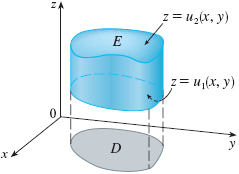
\includegraphics[width=6cm]{12_5_2}
  \end{center}

  If $ E $ is a Type 1 region, then we can calculate the volume of $ E $ like so
  \[
    \INT*{^{},_E,^{}}f(x,y,z)=\INT*{^{},_D} \text{\huge{[}} \int^{u_2(x,y)}_{u_1(x,y)} f(x,y,z)~dz \text{\huge{]}}dA
  \]

  The meaning of the inner integral on the right side is that $ x ~\&~ y $ are  held fixed, and therefore $ u_1(x,y) ~\&~ u_2(x,y) $ are regarded as constants, while $ f(x,y,z) $ is integrated with respect to $ z $.

  In particular if the projection $ D $ of $ E $ onto the $ xy $ plane is a Type I plane region (as in the figure below), then
  \[
    E = \{ (x,y,z) | a \le x \le b, g_1(x) \le y \le g_2(x), u_1(x,y) \le z \le u_2(x,y) \}
  \]
 
  Giving us
  \[
    \INT*{^{},_E,^{}} f(x,y,z)~dV = \int^{b}_{a} \int^{g_2(x)}_{g_1(x)} \int^{u_2(x,y)}_{u_1(x,y)} f(x,y,z) ~ dzdydx
  \]

  \begin{center}
    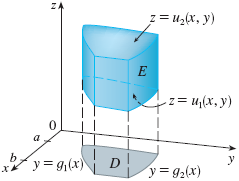
\includegraphics[width=6cm]{12_5_3}
  \end{center}

  However if $ D $ is a Type II plane region like the figure below, then
  \[
    E = \{ (x,y,z) | c \le y \le d, h_1(y) \le y \le h_2(y),u_1(x,y) \le z \le u_2(x,y) \}
  \]

  Which gives
  \[
    \INT*{^{},_E,^{}}f(x,y,z)~dV = \int^{d}_{c} \int^{h_2(y)}_{h_1(y)} \int^{u_2(x,y)}_{u_1(x,y)} f(x,y,z) ~ dzdydx
  \]

  \begin{center}
    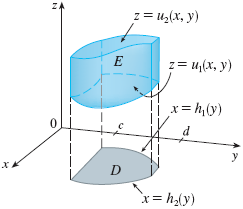
\includegraphics[width=6cm]{12_5_4}
  \end{center}

  A Type I solid region with a Type II projection is shown in the figure above.

  \textbf{Ex 2}\\
  Evaluate $ \INT*{^{},_E,^{}} z~dV$, where $ E $ is the solid tetrahedron bounded by the four planes $ x=0,y=0, ~\&~ x+y+z=1 $.

  \begin{center}
    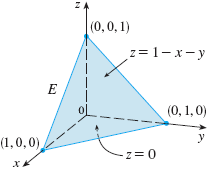
\includegraphics[width=6cm]{12_5_5}
    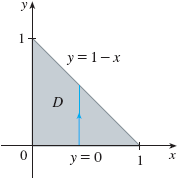
\includegraphics[width=5cm]{12_5_6}
  \end{center}

  After sketching out the solid and region, we find that
  \[
    \begin{gathered}
    E=\{ (x,y,z) | 0 \le x \le 1, 0 \le y \le 1-x, 0 \le z \le 1 -x -y \}\\
    ~\\
    \INT*{^{},_E,^{}}z~dV = \int^{1}_{0} \int^{1-x}_{0} \int^{1-x-y}_{0} z ~ dzdydx\\
    \int^{1}_{0} \int^{1-x}_{0} \text{\huge{[}} \frac{z^{2}}{2} \text{\huge{]}}^{z=1-x-y}_{z=0} ~ dydx\\
    \frac{1}{2} \int^{1}_{0} \int^{1-x}_{0} (1-x-y)^{2} ~ dydx\\
    \frac{1}{2} \int^{1}_{0} \text{\huge{[}} -\frac{(1-x-y)^{3}}{3} \text{\huge{]}}^{y=1-x}_{y=0}~dx\\
    \frac{1}{6} \int^{1}_{0} (1-x)^{3}~dx=\frac{1}{6} \text{\huge{[}} -\frac{(1-x)^{4}}{4} \text{\huge{]}}^{1}_0=\boxed{\frac{1}{24}}
    \end{gathered}
  \]

  A solid region $ E $ is of Type II if it is of the form
  \[
    E=\{ (x,y,z) | (y,z) \in D, u_1(y,z) \le x \le u_2(y,z) \}
  \]
  
  Where $ D $ is the projection of $ E $ onto the $ yz $ plane. The back surface is $ x=u_1(y,z) $, as shown below

  \begin{center}
    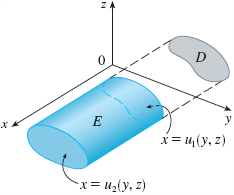
\includegraphics[width=5cm]{12_5_7}
  \end{center}

  Which gives
  \[
    \INT*{^{},_E,^{}}f(x,y,z)~dV= \INT*{^{},_D} \text{\huge{[}} \int^{u_2(y,z)}_{u_1(y,z)} f(x,y,z)~dx \text{\huge{]}}~dA
  \]
  
  Finally, a Type III region is of the form
  \[
    E=\{ (x,y,z) | (x,z) \in D,u_1(x,z) \le y \le u_2(x,z)\}
  \]

  Where $ D $ is the projection of $ E $ onto the $ xz $ plane, $ y=u_1(x,z) $ is the left surface and $ y=u_2(x,z) $ is the right surface.
  
  \begin{center}
    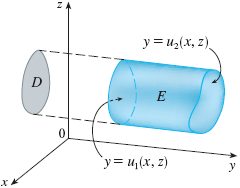
\includegraphics[width=5cm]{12_5_8}
  \end{center}

  \[
    \INT*{^{},_E,^{}} f(x,y,z)~dV = \INT*{^{},_D} \text{\huge{[}} \int^{u_2(x,z)}_{u_1(x,z)} f(x,y,z)~dy \text{\huge{]}}~dA
  \]
 
  In each of the equations for Type II and Type III regions, there may be two possible expressions for the integral depending on whether $ D $ is a Type I or Type II plane region.

  \textbf{Ex 3}\\
  Evaluate $ \iiint_E \sqrt{x^{2}+z^{2}} ~dV $, where $ E $ is the region bounded by the paraboloid $ y=x^{2}+z^{2} $ and the plane $ y=4 $.
  \begin{center}
    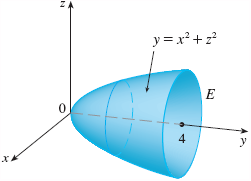
\includegraphics[width=5cm]{12_5_9} 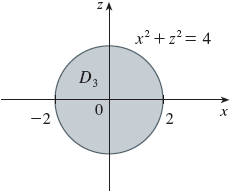
\includegraphics[width=5cm]{12_5_10}
  \end{center}

  We can view the solid $ E $ as a Type III region with its projection $ D $ being on the $ xz $ plane. That is the upper and lower bounds of $ y $ are $ y=4 ~\&~ y=x^{2}+z^{2} $ respectively.$ D $ is also the disk $ x^{2}+z^{2} \le 4 $ based on our boundaries set for $ y $. We can get the region
  \[
    E=\{ (x,z) | -2 \le x \le 2, -\sqrt{4-x^{2}} \le z \le \sqrt{4-x^{2}}, x^{2}+z^{2} \le y \le 4   \}
  \]
  
  \[
    \begin{gathered}
      \INT*{^{},_E,^{}} \sqrt{x^{2}+z^{2}}~dV = \INT*{^{},_D} \text{\huge{[}} \int^{4}_{x^{2}+z^{2}} \sqrt{x^{2}+z^{2}}  ~dy \text{\huge{]}}~dA\\
      \INT*{^{},_D}(4-x^{2}-z^{2})\sqrt{x^{2}+z^{2}}~dA\\
      \int^{2}_{-2} \int^{\sqrt{4-x^{2}}}_{-\sqrt{4-x^{2}}}(4-x^{2}-z^{2})\sqrt{x^{2}+z^{2}} ~dzdx  
    \end{gathered}
  \]

  Due to the circular nature of the $ xz $ plane, we can also convert to polar coordinates.
  \[
    \begin{gathered}
      \int^{2}_{-2} \int^{\sqrt{4-x^{2}}}_{-\sqrt{4-x^{2}}}(4-x^{2}-z^{2})\sqrt{x^{2}+z^{2}} ~dzdx=\int^{2\pi}_{0} \int^{2}_{0}(4-r^{2})\sqrt{r^{2}}r ~drd\theta\\
        \int^{2\pi}_{0} \int^{2}_{0}4r^{2}-r^{4} ~drd\theta\\
        \int^{2\pi}_{0} d\theta \int^{2}_{0} 4r^{2}-r^{2} ~dr = 2\pi \text{\huge{[}} \frac{4r^{3}}{3}-\frac{r^{5}}{5} \text{\huge{]}}^{2}_0=\boxed{\frac{128\pi}{15}}
    \end{gathered}
  \] 

  \textbf{Applications of Triple Integrals}\\
  If the density function of a solid object that occupies the region $ E $ is $ \rho(x,y,z) $, in units of mass per unit voume, at any given point $ (x,y,z) $, then its mass is
  \[
    m=\INT*{^{},_E,^{}} \rho(x,y,z)~dV
  \]

  So its moments about the three coordinate planes
  are
  \[
    \begin{gathered}
      M_{yz} = \INT*{^{},_E,^{}} x\rho(x,y,z)~dV \qquad
      M_{xz} = \INT*{^{},_E,^{}} y\rho(x,y,z)~dV \qquad
      M_{xy} = \INT*{^{},_E,^{}} z\rho(x,y,z)~dV
    \end{gathered}
  \]

  The center of mass is located at the point $ (\overline{x},\overline{y},\overline{z}) $, where
  \[
    \overline{x}=\frac{M_{yz}}{m} \qquad
    \overline{y}=\frac{M_{xz}}{m} \qquad
    \overline{y}=\frac{M_{xy}}{m}
  \]

  If the density is constant, the center of mass of the solid is called the centroid of $ E $. The moments of inertia about the three coordinate axes are
  \[
    \begin{gathered}
      I_x = \INT*{^{},_E,^{}} (y^{2}+z^{2}) \rho(x,y,z)~dV \qquad
      I_y = \INT*{^{},_E,^{}} (x^{2}+z^{2}) \rho(x,y,z)~dV \\
      I_z = \INT*{^{},_E,^{}} (x^{2}+y^{2}) \rho(x,y,z)~dV 
    \end{gathered}
  \]
 
  The total electric charge on a solid object occupying a region $ E $ and having charge density $ \rho(x,y,z) $ is
  \[
    Q= \INT*{^{},_E,^{}} \sigma(x,y,z)~dV
  \]
  
  \textbf{Ex 6}\\
  Find the center of mass of a solid of constant density that is bounded by the parabolic cylinder $ x=y^{2} $ and the planes $ x=z,z=0, ~\&~ x=1 $.

  \begin{center}
    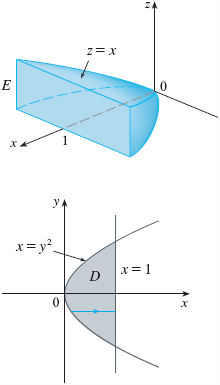
\includegraphics[width=4cm]{12_5_11}
  \end{center}

  \[
    \begin{gathered}
      m=\INT*{^{},_E,^{}} \rho~dV = \int^{1}_{-1} \int^{1}_{y^{2}} \int^{x}_{0} \rho  ~dV = \frac{4\rho}{5} 
    \end{gathered}
  \]

  Since $ E ~\&~ \rho $ is symmetrical about the $ xz $ plane, we can sa that $ M_{xz}=0 $ and therefore $ \overline{y}=0 $. 
  \[
    \begin{gathered}
      M_{yz} = \INT*{^{},_E,^{}}x\rho~dV = \int^{1}_{-1} \int^{1}_{y^{2}} \int^{x}_{0} x\rho ~ dzdxdy = \frac{4\rho}{7}\\
      M_{xy}=\INT*{^{},_E,^{}} z\rho~dV= \int^{1}_{-1} \int^{1}_{y^{2}} \int^{x}_{0} z\rho ~ dzdxdy =\frac{2\rho}{7}\\
      ~\\
      (\overline{x},\overline{y},\overline{z}) = (\frac{M_{yz}}{m},\frac{M_{xz}}{m},\frac{M_{xy}}{m}) = \boxed{(\frac{5}{7}),0,\frac{5}{14}}
    \end{gathered}
  \]


\end{document}
